\documentclass[a4paper, 10pt]{article}

% import packages
\usepackage[margin=0.2cm]{geometry}
\usepackage{pdflscape}
\usepackage{array}
\usepackage{makecell}
\usepackage{xcolor}
\usepackage{colortbl}
\usepackage{longtable}
\usepackage{titlesec}
\usepackage{float}
\usepackage{needspace}
\usepackage{graphicx}
\usepackage{hyperref}
\usepackage{setspace}
\usepackage{fancyhdr}
\usepackage{enumitem}
\usepackage{multicol}
\usepackage{amsmath}
\usepackage{graphicx}
\usepackage[table]{xcolor}
\usepackage{booktabs}   % for \toprule, \midrule, \bottomrule
\usepackage{adjustbox}  % for \begin{adjustbox}{max width=\textwidth}
\usepackage{etoolbox}
\usepackage{tikz}
\usetikzlibrary{arrows.meta, positioning, shapes.geometric}

\AtBeginEnvironment{tabular}{\tiny}

\renewcommand{\familydefault}{\sfdefault}

\newlength\tindent
\setlength{\tindent}{\parindent}
\setlength{\parindent}{0pt}
\renewcommand{\indent}{\hspace*{\tindent}}

% global list spacing (affects all levels)
\setlist{noitemsep, topsep=0pt, parsep=0pt, partopsep=0pt}

% now explicitly override indentation for each level you care about:
\setlist[itemize,1]{leftmargin=1.8em}
\setlist[itemize,2]{leftmargin=1.4em}
\setlist[itemize,3]{leftmargin=0.5em}

% Only change level 1 itemize bullets
\setlist[itemize,1]{label=\raisebox{0.5ex}{\scalebox{0.6}{$\bullet$}}}
%\setlist[itemize,3]{label=\raisebox{0.5ex}{\scalebox{0.6}{$\bullet$}}}

\setlength{\columnseprule}{0.1pt}
% ------------------------------------------------------


% Configure makecell package
\renewcommand{\theadalign}{bc}
\renewcommand{\theadgape}{\Gape[4pt]}
\renewcommand{\cellgape}{\Gape[4pt]}
\renewcommand{\cellalign}{lt}

% global line spacing
\renewcommand{\baselinestretch}{1.2}

% colour definitions
\definecolor{lightergray}{gray}{0.90}

\providecommand{\tightlist}{%
\setlength{\itemsep}{0pt}
\setlength{\parskip}{0pt}}

\begin{document}
  \begin{landscape}

\tiny

\begin{itemize}
    \item \texttt{?} \(\rightarrow\) 0-1
    \item \texttt{*} \(\rightarrow\)  0-n
    \item \texttt{+} \(\rightarrow\) 1-n
    \item \texttt{*?} \(\rightarrow\) 0-n (lazy)
\end{itemize}

\vspace{0.4em}
\hrule
\vspace{0.7em}

{\footnotesize TF-IDF}
\begin{itemize}
    \item 
\end{itemize}

{\scriptsize{Term Frequency TF}}
\(\uparrow\) weight of common words in doc \\
tf(term,doc) = \# times term in doc / total \# of terms in doc

\vspace{-12pt}
\begin{table}[ht]
\begin{adjustbox}{max width=\textwidth}
\setlength{\tabcolsep}{1pt}      % default is ~6pt
\renewcommand{\arraystretch}{0.5} % default is 1.0
\begin{tabular}{l|r|r|r|r|r|r|r|r|r}
\midrule
\textbf{sentence} 
& \textbf{a} & \textbf{cat} & \textbf{dog} & \textbf{is} & \textbf{it} 
& \textbf{my} & \textbf{not} & \textbf{old} & \textbf{wolf} \\
\midrule
\textit{``It is a dog.''} & 0.25 & 0 & 0.25 & 0.25 & 0.25 & 0 & 0 & 0 & 0 \\
\textit{``my cat is old''} & 0 &  0.25 & 0 & 0.25 & 0 & 0.25 & 0 & 0.25 & 0 \\
\textit{``It is not a dog, it a is wolf.''} & 0.22 & 0 & 0.11 & 0.22 & 0.22 & 0 & 0.11 & 0 & 0.11 \\
\midrule
\end{tabular}
\end{adjustbox}
\end{table}
\vspace{-11pt}

{\scriptsize{Inverse Document Frequency IDF}}
\(\downarrow\) weight for common words \(\uparrow\) weights for rare words

idf(term) = log(\# docs / \# docs with term)

\vspace{-12pt}
\begin{table}[ht]
\begin{adjustbox}{max width=\textwidth}
\setlength{\tabcolsep}{1pt}      % default is ~6pt
\renewcommand{\arraystretch}{0.5} % default is 1.0
\begin{tabular}{l|l}
\midrule
\textbf{term} & \textbf{idf} \\
\midrule
a & log(3/2) = 0.17 \\
cat & log(3/1) = 0.47 \\
dog & log(3/2) = 0.17 \\
is & log(3/3) = 0 \\
my & log(3/1) = 0.47 \\
.. & .. \\
\end{tabular}
\end{adjustbox}
\end{table}
\vspace{-11pt}

{\scriptsize{TF-IDF}} tf-idf(term,doc) = tf(term,doc) * idf(term) 

{\scriptsize{Query}} 
\textbf{"cat is wolf"} 
If one words appears eg. 2 times in query, score is multiplied by 2
\vspace{-12pt}
\begin{table}[ht]
\begin{adjustbox}{max width=\textwidth}
\setlength{\tabcolsep}{1pt}      % default is ~6pt
\renewcommand{\arraystretch}{0.5} % default is 1.0
\begin{tabular}{l|r|r|r|r|r|r|r|r|r||rr}
\midrule
\textbf{sentence} 
& \textbf{a} & \textbf{cat} & \textbf{dog} & \textbf{is} & \textbf{it} 
& \textbf{my} & \textbf{not} & \textbf{old} & \textbf{wolf} 
& \textbf{score} & \textbf{rank} \\
\midrule
\textit{``It is a dog.''} 
& 0.044 &  & 0.044 & \cellcolor{yellow} 0 &  0.044 &  &  &  & & 0 & - \\
\textit{``my cat is old''} 
& & \cellcolor{yellow} 0.119 & & \cellcolor{yellow} 0 & & 0.199 &  & 0.119 & & 0.119 & 1 \\
\textit{``It is not a dog, it a is wolf.''} 
& 0.039 &  & 0.02 & \cellcolor{yellow} 0 & 0.039 &  & 0.053 &  & \cellcolor{yellow} 0.053 & 0.053 &  2 \\
\midrule
\end{tabular}
\end{adjustbox}
\end{table}
\vspace{-11pt}


\vspace{0.4em}
\hrule
\vspace{0.7em}

{\footnotesize Attention (Transformer Core)}

\begin{itemize}
    \item \textbf{which parts of a sequence matter most} for each token
    \item Instead of reading strictly left-to-right, attention lets each token measure its \textbf{relevance to other tokens} and build a \textbf{context-aware representation}.
    \item models \textbf{token-to-token relevance}
    \item strengthens \textbf{important context}
    \item creates each output token as a \textbf{weighted combination of previous tokens}
\end{itemize}

\textbf{Example:}  
Sentence: \textit{``The animal didn't cross the street because it was tired.''}  
The token \textbf{``it''} should attend strongly to \textbf{``animal''} (not \textbf{street}), because that resolves the meaning.

\vspace{0.4em}

{\footnotesize Self-Attention}

In \textbf{self-attention}, each token can “look at” \textbf{all other tokens} (including itself). This allows the model to capture:
\begin{itemize}
    \item \textbf{local dependencies} (nearby words)
    \item \textbf{long-range dependencies} (far relationships)
    \item richer \textbf{contextual embeddings}
\end{itemize}

Self-attention produces \textbf{new embeddings} that are more informative than the input embeddings.

\textbf{Example (long-range dependency):}  
\textit{``The book that the professor recommended was expensive.''}  
The token \textbf{``was''} must attend to \textbf{``book''} (the true subject), even though they are far apart.

\vspace{0.4em}
{\footnotesize Query / Key / Value (Q / K / V)}

Each token is projected (via learned weight matrices) into three vectors:
\begin{itemize}
    \item \textbf{Query (Q):} what the current token is looking for
    \item \textbf{Key (K):} what each token offers as “matchable information”
    \item \textbf{Value (V):} the information each token contributes if selected
\end{itemize}

\textbf{Quick intuition:}  
\textbf{Query} = “What do I need?”  
\textbf{Key} = “What do I contain?”  
\textbf{Value} = “What information do I pass on if chosen?”

\textbf{Example:}  
Sentence: \textit{``Alice gave Bob her book.''}  
For token \textbf{``her''}:  
\begin{itemize}
    \item Query asks: “Whose?”  
    \item Keys from \textbf{Alice}, \textbf{Bob} compete as possible owners  
    \item Attention weight becomes larger for \textbf{Alice}, so \textbf{``her''} mixes more of Alice’s value vector.
\end{itemize}

{\scriptsize How it works:}
\begin{enumerate}[leftmargin=1.8em]
    \item Compare current token’s query with all keys:
    \(Q \cdot K^\top\)
    \item Scale scores by $\sqrt{d_k}$ to keep values stable
    \item Apply a \textbf{mask} (for causal models) to block future tokens
    \item Apply \textbf{softmax} to get attention weights
    \item Compute weighted sum of values:
    \( \text{weights} \times V \rightarrow \text{context output} \)
\end{enumerate}

\textbf{Mask example (causal language model):}  
In \textit{``I eat pizza''}, when predicting \textbf{``eat''}, the model may attend to \textbf{``I''} but cannot attend to \textbf{``pizza''}, because it lies in the future.

\textbf{Key insight:}  
Each token becomes a weighted mixture of \textit{all} value vectors, where weights depend on how well the query matches the keys.

\vspace{0.4em}
\hrule
\vspace{0.7em}

{\footnotesize Multi-Head Attention (MHA)}

Transformers run \textbf{multiple self-attention heads in parallel}. Each head has its own learned projection matrices:
\(Q = XW_Q,\quad K = XW_K,\quad V = XW_V\)

This allows each head to learn a different alignment rule over the same input.

\vspace{0.3em}
\textbf{Why multiple heads?}

A single attention head produces only \textbf{one attention pattern} --- a limited view. With multiple heads, the model can attend to different kinds of relationships \textbf{simultaneously}.

Heads often specialize in:
\begin{itemize}
    \item syntax (subject--verb, nearby dependencies)
    \item semantics (topic/meaning connections)
    \item coreference (pronouns $\rightarrow$ entities)
    \item local vs long-range patterns (short vs far dependencies)
\end{itemize}

\vspace{0.3em}
\textbf{How it works (high level)}

Each head computes scaled dot-product attention:
\(
\text{Attention}(Q,K,V)=\text{softmax}\left(\frac{QK^\top}{\sqrt{d_k}}\right)V
\)

Outputs from all heads are:
\begin{itemize}
    \item \textbf{concatenated} (wider feature space)
    \item passed through a \textbf{final linear projection} $W_O$ to mix information back into $d_{\text{model}}$
\end{itemize}

\vspace{0.3em}
\textbf{Example:}  
Sentence: \textit{``The scientist who won the award wrote a paper.''}

\begin{itemize}
    \item One head may link \textbf{``scientist''} $\rightarrow$ \textbf{``wrote''} (grammatical dependency)
    \item Another head may focus inside \textbf{``who won the award''} (relative clause)
    \item Another head may connect \textbf{``won''} $\leftrightarrow$ \textbf{``award''} (semantic association)
\end{itemize}

\textbf{Key idea:}  
Each head is a different perspective on the same sentence --- combining them produces richer token representations.

\vspace{0.4em}
\hrule
\vspace{0.7em}



{\footnotesize Transformer Language Model (Decoder-Style)}

A decoder-style transformer is designed for \textbf{next-token prediction}. It uses self-attention with a causal mask so that each token can only attend to earlier positions.

\begin{itemize}
    \item \textbf{Masked self-attention:} prevents future information leakage  
    (token at position $t$ can only attend to positions $\leq t$)
    \item \textbf{Positional encoding:} attention has no built-in notion of order, so positional information is injected into embeddings (sinusoidal or learned)
    \item \textbf{Feed-forward network (FFN):} applied independently to each token, expanding and compressing dimensions:
    \(
    d_{\text{model}} \rightarrow d_{\text{ff}} \rightarrow d_{\text{model}}
    \)
    adds nonlinearity beyond attention
    \item \textbf{Residual connections:} input is added back after each sublayer (skip connections), improving gradient flow and enabling deep stacking
    \item \textbf{Layer normalization:} stabilizes training by controlling activation scale and improving convergence
\end{itemize}

\vspace{0.4em}
\hrule
\vspace{0.7em}



{\footnotesize Transformer Architecture (Stacked Blocks)}

A transformer is built by stacking many identical \textbf{decoder blocks}.

\vspace{0.3em}
\textbf{One transformer block (decoder)}

In the \textbf{Pre-Norm} version (common in modern models):
\begin{itemize}
    \item LayerNorm $\rightarrow$ Masked MHA $\rightarrow$ Residual add
    \item LayerNorm $\rightarrow$ FFN $\rightarrow$ Residual add
\end{itemize}

Pre-Norm means normalization happens \textbf{before} each sublayer:
\begin{itemize}
    \item improves stability in deep transformers
    \item avoids gradient issues seen in post-norm designs
\end{itemize}

\vspace{0.3em}
\textbf{Why stacking many blocks matters}

Representations become increasingly abstract across layers:
\begin{itemize}
    \item \textbf{Lower layers:} token identity, local syntax
    \item \textbf{Middle layers:} phrase structure, grammatical relations, semantic grouping
    \item \textbf{Higher layers:} long-range dependencies, high-level meaning, prediction-ready features
\end{itemize}

Finally, the output is mapped through a linear layer and softmax to produce the \textbf{next-token probability distribution}.

\vspace{0.4em}
\hrule
\vspace{0.7em}

\textcolor{red}{Sample Exam Questions}

Explain the progression from Bag-of-Words to learned embeddings:
a) What are the key limitations of binary Bag-of-Words representations? (List at least 3)
b) How do learned embeddings address these limitations?
A student says: "Why do we need attention? RNNs already have memory through their hidden state."
a) Explain the fundamental bottleneck problem with RNNs when processing long sequences.
b) Draw a simple diagram showing how information flows in:
– An RNN processing a 10-word sentence
– A transformer with attention processing the same sentence
The Three Representations of Text
– Across episodes, we saw three ways to represent text. 
– For each, explain when and why it's useful: Binary BoW; Dense Embeddings; Contextualized (Transformer)

\vspace{0.4em}
\hrule
\vspace{0.7em}



\vspace{0.7em}

{\footnotesize{Attention}}

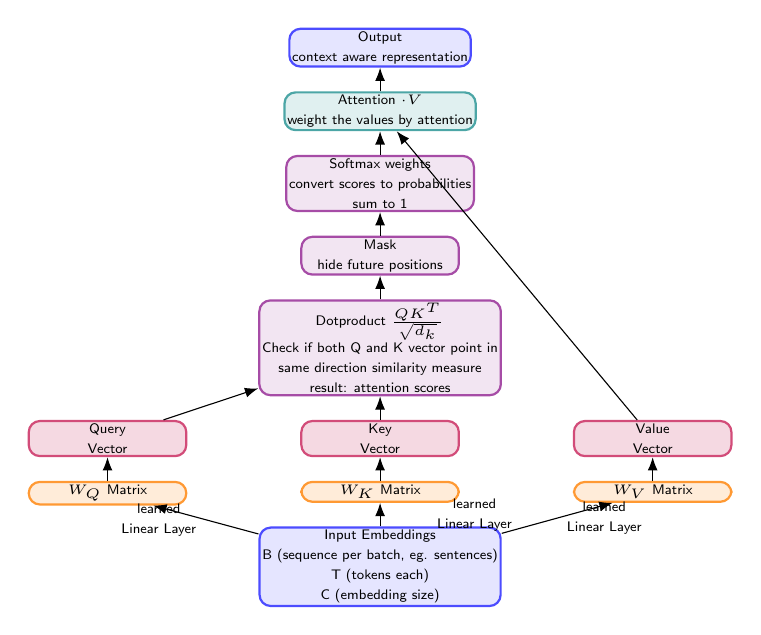
\begin{tikzpicture}[
  node distance=3mm and 5mm,
  >=Latex,
  font=\tiny,
  block/.style={
    rectangle, rounded corners,
    draw, thick, align=center,
    inner sep=1pt,              % <<< less padding
    minimum width=2cm,          % <<< smaller nodes
    % minimum height=7mm
  },
  input/.style={block, fill=blue!10, draw=blue!70},
  proj/.style={block, fill=orange!15, draw=orange!80},
  vec/.style={block, fill=purple!15, draw=purple!70},
  mid/.style={block, fill=violet!10, draw=violet!70},
  att/.style={block, fill=teal!12, draw=teal!70},
]

% --- Output ---
\node[input] (OUT) {Output\\ context aware representation};

% --- Weighted sum ---
\node[att, below=of OUT] (AV) {Attention $\cdot V$\\ weight the values by attention};

% --- Softmax / Mask / Score ---
\node[mid, below=of AV] (SM) {Softmax weights\\ convert scores to probabilities\\ sum to 1};
\node[mid, below=of SM] (MASK) {Mask\\ hide future positions};
\node[mid, below=of MASK] (SCORE) {Dotproduct $\frac{QK^T}{\sqrt{d_k}}$\\ Check if both Q and K vector point in \\same direction similarity measure\\result: attention scores};

% --- Q / K / V ---
\node[vec, below left=of SCORE, xshift=-4mm] (Q) {Query\\ Vector};
\node[vec, below=of SCORE] (K) {Key\\ Vector};
\node[vec, below right=of SCORE, xshift=4mm] (V) {Value\\ Vector};

% --- Projection matrices ---
\node[proj, below=of Q] (WQ) {$W_Q$ Matrix};
\node[proj, below=of K] (WK) {$W_K$ Matrix};
\node[proj, below=of V] (WV) {$W_V$ Matrix};

% --- Input ---
\node[input, below=of WK] (IN) {Input Embeddings\\
B (sequence per batch, eg. sentences)\\
T (tokens each)\\
C (embedding size)};

% --- Arrows ---
\draw[->] (IN) -- node[left, align=center] {learned\\ Linear Layer} (WQ);
\draw[->] (IN) -- node[right, align=center] {learned\\ Linear Layer} (WV);
\draw[->] (IN) -- node[midway, right, align=center, xshift=6mm] {learned\\ Linear Layer} (WK);

\draw[->] (WQ) -- (Q);
\draw[->] (WK) -- (K);
\draw[->] (WV) -- (V);

\draw[->] (Q) -- (SCORE);
\draw[->] (K) -- (SCORE);

\draw[->] (SCORE) -- (MASK);
\draw[->] (MASK) -- (SM);

\draw[->] (SM) -- (AV);
\draw[->] (V) -- (AV);

\draw[->] (AV) -- (OUT);

\end{tikzpicture}

{\footnotesize{Multi Head Attention}}

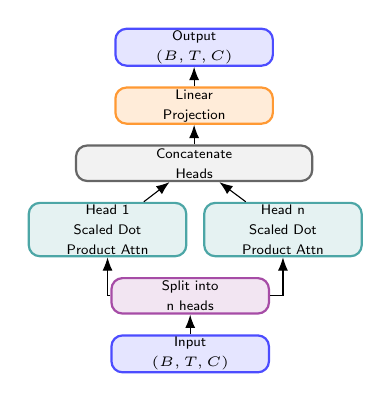
\begin{tikzpicture}[
  node distance=2.5mm and 3.5mm,   % <<< tighter overall
  >=Latex,
  font=\tiny,
  block/.style={
    rectangle, rounded corners,
    draw, thick, align=center,
    inner sep=0.7pt,
    minimum height=4.5mm,
    minimum width=2.0cm
  },
  wide/.style={
    block,
    minimum width=3.0cm
  },
  input/.style={block, fill=blue!10, draw=blue!70},
  mid/.style={block, fill=violet!10, draw=violet!70},
  head/.style={block, fill=teal!10, draw=teal!70},
  concat/.style={wide, fill=gray!10, draw=black!60},
  proj/.style={block, fill=orange!15, draw=orange!80},
]

% --- Top / output ---
\node[input] (OUT) {Output\\ $(B,T,C)$};

% --- Final projection + concat ---
\node[proj, below=of OUT] (WO) {Linear\\ Projection};
\node[concat, below=of WO] (CAT) {Concatenate\\ Heads};

% --- Heads: explicitly placed close together ---
\node[head, below=of CAT, xshift=-1.1cm] (H1) {Head 1\\ Scaled Dot\\ Product Attn};
\node[head, right=2mm of H1] (H2) {Head n\\ Scaled Dot\\ Product Attn};

% --- Split + input ---
\node[mid, below=of H1, xshift=1.05cm] (SPLIT) {Split into\\ n heads};
\node[input, below=of SPLIT] (IN) {Input\\ $(B,T,C)$};

% --- Arrows (BT) ---
\draw[->] (IN) -- (SPLIT);

\draw[->] (SPLIT) -| (H1);
\draw[->] (SPLIT) -| (H2);

\draw[->] (H1) -- (CAT);
\draw[->] (H2) -- (CAT);

\draw[->] (CAT) -- (WO);
\draw[->] (WO) -- (OUT);

\end{tikzpicture}




\end{landscape}
\end{document}